\newpage
  \begin{tikzpicture}[remember picture,overlay]
    % Default apex angle 30 degrees
    \node(bottom-rectangle)[rectangle,
        fill=Light-Gray, minimum height=5cm, minimum width=2\textwidth] () at (current page.north)
        {};
    
    \node(left-triagle)[isosceles triangle,
        isosceles triangle apex angle=90,
        fill=Light-Gray,
        minimum size =0.4\textheight] (T.west) at (current page.north west){};

    \node(bottom-rectangle)[rectangle,
        fill=Light-Gray, minimum height=5cm, minimum width=2\textwidth] () at (current page.south)
        {};

    \node(left-triagle)[isosceles triangle,
        isosceles triangle apex angle=90, rotate=90,
        fill=Light-Gray,
        minimum size =0.4\textheight] (T.west) at (current page.south east){};


    \node[inner sep=0pt, anchor=west] (logo) at ([xshift=1.2cm, yshift=-1.5cm]current page.north west)
    {
\includegraphics[width= 0.4\textwidth]{Figures/PP-PUT-WORD.png}};

    \node[inner sep=0pt, anchor=center] (logo2) at ([xshift=-1.6cm, yshift=1.7cm]current page.south east)
    {
\includegraphics[width= 2.2cm]{Figures/PP-PUT-WIIT-LOGO.png}};


    \draw [double distance=4mm,
           double=gray,
           draw opacity=0,
           rotate=150,
           anchor=center,
           postaction={
                decorate,
                decoration={
                      raise=-1ex,
                      text along path, 
                      reverse path,
                      text align={fit to path stretching spaces},
                      text={|\ttfamily\footnotesize\color{black}|Kierunek\space Informatyka\space |\ttfamily\footnotesize\color{gray}|Wydzial\space Informatyki\space i\space Telekomunikacji}
                }
           }
        ] (logo2.center) circle (1.4cm);
    
  \end{tikzpicture}
\newtcblisting{TcblistingMintedPython}[0]{listing engine=minted,minted style=native,
    minted language=python,enhanced,
    minted options={fontsize=\tiny},  
    colback=terminalColor,
    colframe=terminalColor,
    listing only,
    title= \tikz {
        \node[circle,inner sep=0pt] at (0,0){
\includegraphics[width=0.2cm]{Figures/PYTHON-LOGO.png}};;
    } ~~~~~~Python
}
\section{Operacje na drzewach}

\begin{multicols}{2}
  \begin{enumerate}[series=actions]
    \item \textcolor{PUT-Blue}{\putbf{Wyszukiwanie}} w drzewie elementu o najmniejszej i największej wartości
    \begin{figure} [H]
        \centering
        \newtcblisting{TcblistingMintedTerminal}[0]{listing engine=minted,minted style=native,
    minted language=python,enhanced,
    minted options={fontsize=\tiny},  
    colback=terminalColor,colframe=terminalColor,listing only, title=\tikz {
        \node[circle,fill=Button1,inner sep=3pt] (c) at (0,0){};
        \node[circle,fill=Button2,inner sep=3pt] (c) at (0.5,0){};
        \node[circle,fill=Button3,inner sep=3pt] (c) at (1,0){};
    } ~~~~~~Terminal
}

\newenvironment{TikzTreeStyle}
{ % Create enviroment - a tikzpicture with my styling for nodes
    \begin{tikzpicture}
        [level distance=10mm,
        every node/.style={fill=red!60,circle,inner sep=1pt, minimum size=6mm},
        level 1/.style={sibling distance=20mm,nodes={fill=red!45}},
        level 2/.style={sibling distance=10mm,nodes={fill=red!30}},
        level 3/.style={sibling distance=5mm,nodes={fill=red!25}}]
}
{ % Close enviroment
    \end{tikzpicture}
}

\begin{TcblistingMintedTerminal}
>>>  ./program --tree AVL <<< 2, 5, 10, 12, 13, 6, 9
Sorted: 2, 5, 6, 9, 10, 12, 13
Median: 9
action> FindMinMax
Min: 2
Max: 13
\end{TcblistingMintedTerminal}

\begin{TikzTreeStyle}
  \node {9}
    child {node {5} edge from parent [draw=green]
      child {node {2} edge from parent [draw=green] }
      child {node {6} edge from parent [draw=black] }
    }
    child {node {12} edge from parent [draw=red]
      child {node {10} edge from parent [draw=black] }
      child {node {13} edge from parent [draw=  red] }
    };
\end{TikzTreeStyle} 
        \caption{Wyszukiwanie elementu o największej i najmniejszej wartości}
        \label{fig:tree:search}
    \end{figure}
    
    \item \textcolor{PUT-Blue}{\putbf{Wypisanie}} wszystkich elementów drzewa w porządku in-order, pre-order oraz post-order. [Dla chętnych] wypisanie drzewa do tickzpicture
    \begin{figure} [H]
        \centering
        \newtcblisting{TcblistingMintedTerminal}[0]{listing engine=minted,minted style=native,
    minted language=python,enhanced,
    minted options={fontsize=\tiny},  
    colback=terminalColor,colframe=terminalColor,listing only, title=\tikz {
        \node[circle,fill=Button1,inner sep=3pt] (c) at (0,0){};
        \node[circle,fill=Button2,inner sep=3pt] (c) at (0.5,0){};
        \node[circle,fill=Button3,inner sep=3pt] (c) at (1,0){};
    } ~~~~~~Terminal
}

\newenvironment{TikzTreeStyle}
{ % Create enviroment - a tikzpicture with my styling for nodes
    \begin{tikzpicture}
        [level distance=10mm,
        every node/.style={fill=red!60,circle,inner sep=1pt, minimum size=6mm},
        level 1/.style={sibling distance=20mm,nodes={fill=red!45}},
        level 2/.style={sibling distance=10mm,nodes={fill=red!30}},
        level 3/.style={sibling distance=5mm,nodes={fill=red!25}}]
}
{ % Close enviroment
    \end{tikzpicture}
}

\begin{TcblistingMintedTerminal}
action> Print
  In-order:  2,  5,  6,  9, 10, 12, 13
Post-order:  2,  6,  5, 10, 13, 12,  9
 Pre-order:  9,  5,  2,  6, 12, 10, 13
\end{TcblistingMintedTerminal}

\begin{TikzTreeStyle}
  \node {9}
    child {node {5}
      child {node {2} }
      child {node {6} }
    }
    child {node {12}
      child {node {10} }
      child {node {13} }
    };
\end{TikzTreeStyle}
        \caption{Wypisywanie zawartości drzewa (Print)}
        \label{fig:tree:search}
    \end{figure}

    \item \textcolor{PUT-Blue}{\putbf{Narysowanie}} drzewa w tickzpicture \putbf{(dodatkowy punkt)}
    \begin{figure} [H]
        \centering
        \begin{TcblistingMintedPython}
def export():
    if not node.left and not node.right:
        return f"node {node.value}" 
    l_str = f"child {export(node.l)}" if node.l else "child[missing]"
    r_str = f"child {export(node.r)}" if node.r else "child[missing]"
    return f" node {node.value} \{{l_str}\} \{{r_str}\}\"

def main():
    return f"\\{export(tree_root)}"
\end{TcblistingMintedPython}
        \caption{Przykładowa implementacja}
        \label{fig:tree:export:code}
    \end{figure}

    \item \textcolor{PUT-Blue}{\putbf{Usuwanie}} z drzewa ciągu elementów podanych przez użytkownika. Dopuszczalne jest:
    \begin{enumerate}[label=(\alph*)]
        \item usuwanie liści,
        \item usuwanie elementu z jednym potomkiem, 
        \item usuwanie elemntu z dwoma potomkami.
    \end{enumerate}   
    \begin{figure} [H]
        \centering
        \newtcblisting{TcblistingMintedTerminal}[0]{listing engine=minted,minted style=native,
    minted language=python,enhanced,
    minted options={fontsize=\tiny},  
    colback=terminalColor,colframe=terminalColor,listing only, title=\tikz {
        \node[circle,fill=Button1,inner sep=3pt] (c) at (0,0){};
        \node[circle,fill=Button2,inner sep=3pt] (c) at (0.5,0){};
        \node[circle,fill=Button3,inner sep=3pt] (c) at (1,0){};
    } ~~~~~~Terminal
}

\newenvironment{TikzTreeStyle}
{ % Create enviroment - a tikzpicture with my styling for nodes
    \begin{tikzpicture}
        [level distance=10mm,
        every node/.style={fill=red!60,circle,inner sep=1pt, minimum size=6mm},
        level 1/.style={sibling distance=20mm,nodes={fill=red!45}},
        level 2/.style={sibling distance=10mm,nodes={fill=red!30}},
        level 3/.style={sibling distance=5mm,nodes={fill=red!25}}]
}
{ % Close enviroment
    \end{tikzpicture}
}

\begin{TcblistingMintedTerminal}
action> Delete
 nodes> 3
delete> 2 5 10

\end{TcblistingMintedTerminal}

\begin{TikzTreeStyle}
\node[draw=black,dash pattern= on 3pt off 5pt,thick,postaction={draw,red,dash pattern= on 3pt off 5pt,dash phase=4pt,thick}] at (0,0) {9} 
child {node {5}
  child {node {2}}
  child {node [draw=black,dash pattern= on 3pt off 5pt,thick,postaction={draw,green,dash pattern= on 3pt off 5pt,dash phase=4pt,thick}] {6}}
}
child {node {12}
  child {node {10}}
  child {node {13}}
};

\node at (4,0) (c) {6} 
child {node {5}
  child {node {2} }
  child [missing]
}
child {node [draw=black,dash pattern= on 3pt off 5pt,thick,postaction={draw,red,dash pattern= on 3pt off 5pt,dash phase=4pt,thick}] {12}
  child {node [draw=black,dash pattern= on 3pt off 5pt,thick,postaction={draw,green,dash pattern= on 3pt off 5pt,dash phase=4pt,thick}] {10}}
  child {node {13}}
};

\node at (0,-3.5) (b) {6} 
child {node {5}
  child {node {2} }
  child [missing]
}
child {node {10}
  child[missing]
  child {node [draw=black,dash pattern= on 3pt off 5pt,thick,postaction={draw,red,dash pattern= on 3pt off 5pt,dash phase=4pt,thick}] {13}}
};


\node at (4,-3.5) (a) {6} 
child {node {5}
  child {node {2} }
  child [missing]
}
child {node {10}};

%Add arrows
\path[double, draw=black, ->] (1.5,  -1) -- (2.5,  -1);
\path[double, draw=black, ->] (2.4,-2.7) -- (1.6,  -3.2);
\path[double, draw=black, ->] (1.5,-4.5) -- (2.5,-4.5);

\node[draw=none,fill=none] (1) [label=above:{(c)}] at (2,   -1) {};
\node[draw=none,fill=none] (1) [label=above:{(b)}] at (2, -3.2) {};
\node[draw=none,fill=none] (1) [label=above:{(a)}] at (2, -4.5) {};
    
\end{TikzTreeStyle} 
        \caption{Usuwanie elementów}
        \label{fig:tree:search}
    \end{figure}

    \item \textcolor{PUT-Blue}{\putbf{Usunięcie}} całego drzewa element po elemencie metodą post-order 
    \begin{figure} [H]
        \centering
        \newtcblisting{TcblistingMintedTerminal}[0]{listing engine=minted,minted style=native,
    minted language=python,enhanced,
    minted options={fontsize=\tiny},  
    colback=terminalColor,colframe=terminalColor,listing only, title=\tikz {
        \node[circle,fill=Button1,inner sep=3pt] (c) at (0,0){};
        \node[circle,fill=Button2,inner sep=3pt] (c) at (0.5,0){};
        \node[circle,fill=Button3,inner sep=3pt] (c) at (1,0){};
    } ~~~~~~Terminal
}

\newenvironment{TikzTreeStyle}
{ % Create enviroment - a tikzpicture with my styling for nodes
    \begin{tikzpicture}
        [level distance=10mm,
        every node/.style={fill=red!60,circle,inner sep=1pt, minimum size=6mm},
        level 1/.style={sibling distance=20mm,nodes={fill=red!45}},
        level 2/.style={sibling distance=10mm,nodes={fill=red!30}},
        level 3/.style={sibling distance=5mm,nodes={fill=red!25}}]
}
{ % Close enviroment
    \end{tikzpicture}
}

\begin{TcblistingMintedTerminal}
action> Delete All
Deleting: 2 5 10 6
Tree succesfully removed
\end{TcblistingMintedTerminal}


\begin{TikzTreeStyle}
%  _   _                             _            __  _     _____                 
% | | | | _ __   _ __    ___  _ __  | |     ___  / _|| |_  |_   _|_ __  ___   ___ 
% | | | || '_ \ | '_ \  / _ \| '__| | |    / _ \| |_ | __|   | | | '__|/ _ \ / _ \
% | |_| || |_) || |_) ||  __/| |    | |___|  __/|  _|| |_    | | | |  |  __/|  __/
%  \___/ | .__/ | .__/  \___||_|    |_____|\___||_|   \__|   |_| |_|   \___| \___|
%        |_|    |_|                                                               
\node at (0,0)  {6} 
child {node {5}
  child {node [draw=black,dash pattern= on 3pt off 5pt,thick,postaction={draw,red,dash pattern= on 3pt off 5pt,dash phase=4pt,thick}] {2} }
  child [missing]
}
child {node {10}};

%  _   _                             ____   _         _      _     _____                 
% | | | | _ __   _ __    ___  _ __  |  _ \ (_)  __ _ | |__  | |_  |_   _|_ __  ___   ___ 
% | | | || '_ \ | '_ \  / _ \| '__| | |_) || | / _` || '_ \ | __|   | | | '__|/ _ \ / _ \
% | |_| || |_) || |_) ||  __/| |    |  _ < | || (_| || | | || |_    | | | |  |  __/|  __/
%  \___/ | .__/ | .__/  \___||_|    |_| \_\|_| \__, ||_| |_| \__|   |_| |_|   \___| \___|
%        |_|    |_|                            |___/                                     
\node at (4,0) (c) {6} 
child {node [draw=black,dash pattern= on 3pt off 5pt,thick,postaction={draw,red,dash pattern= on 3pt off 5pt,dash phase=4pt,thick}] {5}}
child {node {10}};

%  _                                 _            __  _     _____                 
% | |     ___ __      __ ___  _ __  | |     ___  / _|| |_  |_   _|_ __  ___   ___ 
% | |    / _ \\ \ /\ / // _ \| '__| | |    / _ \| |_ | __|   | | | '__|/ _ \ / _ \
% | |___| (_) |\ V  V /|  __/| |    | |___|  __/|  _|| |_    | | | |  |  __/|  __/
% |_____|\___/  \_/\_/  \___||_|    |_____|\___||_|   \__|   |_| |_|   \___| \___|
%
\node at (0,-3.5) (b) {6} 
child[missing]
child {node [draw=black,dash pattern= on 3pt off 5pt,thick,postaction={draw,red,dash pattern= on 3pt off 5pt,dash phase=4pt,thick}] {10}};

%  _                                 ____   _         _      _     _____                 
% | |     ___ __      __ ___  _ __  |  _ \ (_)  __ _ | |__  | |_  |_   _|_ __  ___   ___ 
% | |    / _ \\ \ /\ / // _ \| '__| | |_) || | / _` || '_ \ | __|   | | | '__|/ _ \ / _ \
% | |___| (_) |\ V  V /|  __/| |    |  _ < | || (_| || | | || |_    | | | |  |  __/|  __/
% |_____|\___/  \_/\_/  \___||_|    |_| \_\|_| \__, ||_| |_| \__|   |_| |_|   \___| \___|
%                                              |___/                                     
\node at (4,-3.5) (a) [draw=black,dash pattern= on 3pt off 5pt,thick,postaction={draw,red,dash pattern= on 3pt off 5pt,dash phase=4pt,thick}] {6};

%%%%%%%%%%%%%%%%%%%%%%%%%%%%%%%%%%%%%%%%%%%%%%%%%%%%%%%%%%%%%%%%%%%%%%%%
%   Add arrows 
%%%%%%%%%%%%%%%%%%%%%%%%%%%%%%%%%%%%%%%%%%%%%%%%%%%%%%%%%%%%%%%%%%%%%%%%
\path[double, draw=black, ->] (1.5,  -1) -- (2.5,  -1);
\path[double, draw=black, ->] (2.4,-2.7) -- (1.6,  -3.2);
\path[double, draw=black, ->] (1.5,-4.5) -- (2.5,-4.5);
    
\end{TikzTreeStyle} 
        \caption{Usuwanie drzewa}
        \label{fig:tree:search}
    \end{figure}

    
  \end{enumerate}
\end{multicols}



\newpage
  \begin{tikzpicture}[remember picture,overlay]
    % Default apex angle 30 degrees
    \node(bottom-rectangle)[rectangle,
        fill=Light-Gray, minimum height=5cm, minimum width=2\textwidth] () at (current page.north)
        {};
    
    \node(left-triagle)[isosceles triangle,
        isosceles triangle apex angle=90,
        fill=Light-Gray,
        minimum size =0.4\textheight] (T.west) at (current page.north west){};

    \node(bottom-rectangle)[rectangle,
        fill=Light-Gray, minimum height=5cm, minimum width=2\textwidth] () at (current page.south)
        {};

    \node(left-triagle)[isosceles triangle,
        isosceles triangle apex angle=90, rotate=90,
        fill=Light-Gray,
        minimum size =0.4\textheight] (T.west) at (current page.south east){};


    \node[inner sep=0pt, anchor=west] (logo) at ([xshift=1.2cm, yshift=-1.5cm]current page.north west)
    {
\includegraphics[width= 0.4\textwidth]{Figures/PP-PUT-WORD.png}};

    \node[inner sep=0pt, anchor=center] (logo2) at ([xshift=-1.6cm, yshift=1.7cm]current page.south east)
    {
\includegraphics[width= 2.2cm]{Figures/PP-PUT-WIIT-LOGO.png}};


    \draw [double distance=4mm,
           double=gray,
           draw opacity=0,
           rotate=150,
           anchor=center,
           postaction={
                decorate,
                decoration={
                      raise=-1ex,
                      text along path, 
                      reverse path,
                      text align={fit to path stretching spaces},
                      text={|\ttfamily\footnotesize\color{black}|Kierunek\space Informatyka\space |\ttfamily\footnotesize\color{gray}|Wydzial\space Informatyki\space i\space Telekomunikacji}
                }
           }
        ] (logo2.center) circle (1.4cm);
    
  \end{tikzpicture}

\begin{enumerate}[resume=actions]
    \item \textcolor{PUT-Blue}{\putbf{Równoważenie}} drzewa element po elemencie metodą DSW

\newtcblisting{TcblistingMintedTerminal}[0]{listing engine=minted,minted style=native,
    minted language=python,enhanced,
    minted options={fontsize=\tiny},  
    colback=terminalColor,colframe=terminalColor,listing only, title=\tikz {
        \node[circle,fill=Button1,inner sep=3pt] (c) at (0,0){};
        \node[circle,fill=Button2,inner sep=3pt] (c) at (0.5,0){};
        \node[circle,fill=Button3,inner sep=3pt] (c) at (1,0){};
    } ~~~~~~Terminal
}

\begin{figure}[H]
    \begin{subfigure}{\textwidth}
\begin{TcblistingMintedTerminal}
>>>  ./program --tree AVL <<< 1, 2, 3, 6, 5, 4, 7
Inserting: 1, 2, 3, 6, 5, 4, 7
action> Rebalance
Pre-Order:  4, 2, 1, 3, 6, 5, 7,
\end{TcblistingMintedTerminal}
        \caption{Interfejs linii komend}
        \label{fig:tree:rebalance:code}
    \end{subfigure}

    \centering
    \begin{subfigure}{\textwidth}
        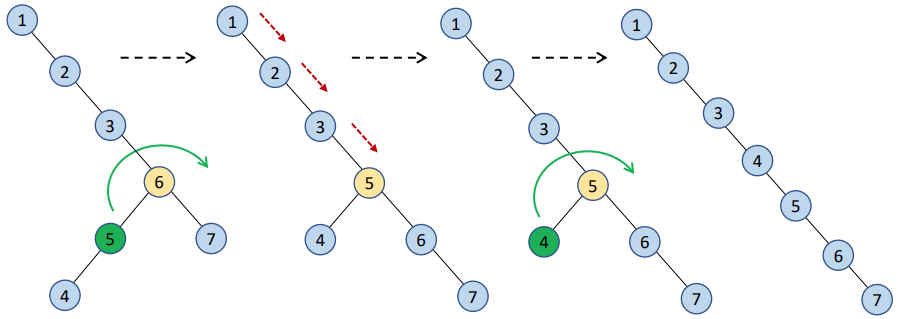
\includegraphics[width=\textwidth]{Figures/DSW-Phase1.png} 
        \caption{Faza pierwsza}
        \label{fig:tree:rebalance:phase1}
    \end{subfigure}

    \begin{subfigure}{\textwidth}
        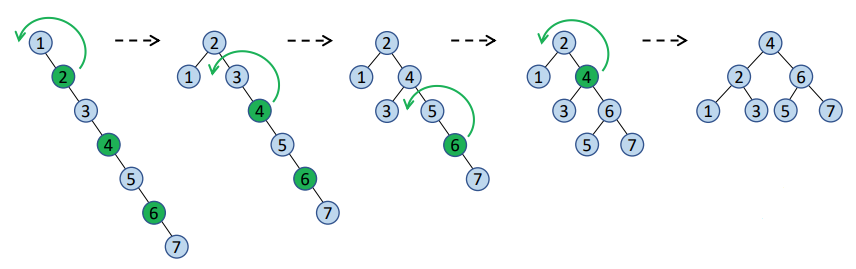
\includegraphics[width=\textwidth]{Figures/DSW-Phase2.png}
        \caption{Faza druga}
        \label{fig:tree:rebalance:phase2}
    \end{subfigure}
    \caption{Równoważenie metodą Day-Stout-Warren}
\end{figure}
    
\end{enumerate}

\section{Wymagania do oceny}
\begin{table}[H]
    \centering
    \begin{tabular}{|c|c|c|c|c|c|c|c|} \hline
    \multicolumn{2}{|c|}{Zadanie 1 - Tworzenie}& Zadanie 2 - Menu         & \multicolumn{5}{c|}{ Zadanie 3 - Operacje              }\\ \hline    
                                     BST & AVL & Zgodność ze specyfikacją & FindMinMax & Print & Remove     & RemoveAll & Rebalance \\ \hline
                                       1 & 3   & 2                        & 1          & 1     & \putbf{4} & 1         & \putbf{7}\\ \hline
    \end{tabular}
    \caption{Szczegółowa Punktacja}
    \label{tab:my_label}
\end{table}
\putbf{W sumie 20 punktów}. Dodatkowe punkty, poza skalą: 1 pkt za export drzewa do tickzpicture. Do 3 punktów za staranność wykonania projketu (np. czystość kodu, ekspertyza w języku czy używanie gita). 

\begin{table}[H]
    \centering
    \begin{tabular}{|c|c|c|c|c|c|c|c|} \hline
         2 & 3     & 3.5   & 4     & 4.5   & 5  & 5.5 \\ \hline
     do 11 & od 12 & od 14 & od 16 & od 18 & 20 & ponad 22\\ \hline
    \end{tabular}
    \caption{Szczegółowa Punktacja}
    \label{tab:my_label}
\end{table}

\newpage
\hspace{1em} % Skip for aesthetics
\section{Benchmark implementacji}
Ponownie przygotuję dla was generator danych wejściowych, które zapiszę do pliku.
Przygotuję też pliki zawierające polecenia które można przekazać do programu.

Tym razem \putbf{to po waszej stronie} leży \putbf{wykonanie pomiar czasu} - dlatego że musimy zmierzyć poszczególne metody, a nie czas trwania wykonywania całego programu. Z racji że mierzymy czas zegarowy, proszę o zrobienie po 4 pomiary i uśrednienie wyniku. Do pomiaru jest:

\begin{enumerate} [label=\putbf{(\alph*)}]
\item tworzenie drzewa AVL metodą połowienia binarnego, 
\item tworzenie drzewa BST poprzez wstawianie kolejno elementów (drzewo zdegnerowane),
\item wyszukiwanie elementów o minimalnej i maksymalnej wartości,
\item wypisywanie wszystkich elementów drzewa (in-order),
\item równoważenia drzewa BST.
\end{enumerate}

Postaram się jeszcze wymyślić sposób aby ułatwić wam mierzenie czasu, ale nie mogę nic obiecać. W razie czego poinformuję was na Discordzie.


  \begin{tikzpicture}[remember picture,overlay]
    % Default apex angle 30 degrees
    \node(bottom-rectangle)[rectangle,
        fill=Light-Gray, minimum height=5cm, minimum width=2\textwidth] () at (current page.north)
        {};
    
    \node(left-triagle)[isosceles triangle,
        isosceles triangle apex angle=90,
        fill=Light-Gray,
        minimum size =0.4\textheight] (T.west) at (current page.north west){};

    \node(bottom-rectangle)[rectangle,
        fill=Light-Gray, minimum height=5cm, minimum width=2\textwidth] () at (current page.south)
        {};

    \node(left-triagle)[isosceles triangle,
        isosceles triangle apex angle=90, rotate=90,
        fill=Light-Gray,
        minimum size =0.4\textheight] (T.west) at (current page.south east){};


    \node[inner sep=0pt, anchor=west] (logo) at ([xshift=1.2cm, yshift=-1.5cm]current page.north west)
    {
\includegraphics[width= 0.4\textwidth]{Figures/PP-PUT-WORD.png}};

    \node[inner sep=0pt, anchor=center] (logo2) at ([xshift=-1.6cm, yshift=1.7cm]current page.south east)
    {
\includegraphics[width= 2.2cm]{Figures/PP-PUT-WIIT-LOGO.png}};


    \draw [double distance=4mm,
           double=gray,
           draw opacity=0,
           rotate=150,
           anchor=center,
           postaction={
                decorate,
                decoration={
                      raise=-1ex,
                      text along path, 
                      reverse path,
                      text align={fit to path stretching spaces},
                      text={|\ttfamily\footnotesize\color{black}|Kierunek\space Informatyka\space |\ttfamily\footnotesize\color{gray}|Wydzial\space Informatyki\space i\space Telekomunikacji}
                }
           }
        ] (logo2.center) circle (1.4cm);
    
  \end{tikzpicture}
\section{Wymagania do sprawozdania}


\begin{itemize}[label={}]
\item \textcolor{PUT-Blue}{[1 pkt]} Zaprezentuj swój program (screenem utworzenia drzewa BST, AVL). Pokaż wizualizację utworzonych wykresów. Drzewo BST ma być niezbalansowane.  

\item \textcolor{PUT-Blue}{[1 pkt]} Na wizualizacjach oznacz liście, korzeń i węzły wewnętrzne.

\item \textcolor{PUT-Blue}{[4 pkt]} Wykonaj 3 wykresy (jeden wykres dla każdej z operacji: tworzenie struktury, wyszukanie min/max, wypisanie in-order) t=f(n) zależności czasu obliczeń t od liczby n elementów w drzewie. Na każdym wykresie przedstaw 2 krzywe - po jednej krzywej dla BST i AVL. 

\item \textcolor{PUT-Blue}{[4 pkt]} Wykonaj wykres t=f(n) zależności czasu równoważenia (t) od liczby elementów (n) w drzewie BST.

\item \textcolor{PUT-Blue}{Dodatkowy: [1 pkt]} Wykonaj sprawozdanie w LaTeXu :)

\item \textcolor{PUT-Blue}{Dodatkowy: [1 pkt]} Przedstaw wykresy w takim ułożeniu:

\begin{figure}[H]
    \centering
    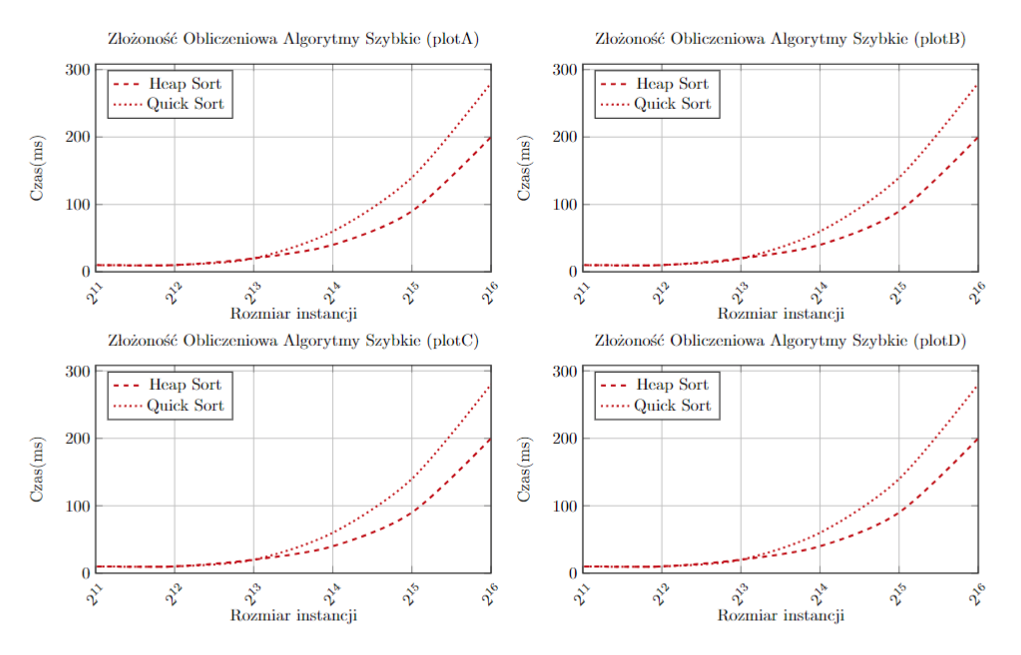
\includegraphics[width=0.4\textwidth]{Figures/Plots.png} 
    \caption{Ilustracja podzielona na 4 podwykresy}
    \label{fig:tree:rebalance:phase1}
\end{figure}

\putbf{W sumie 10 punktów}.
\begin{table}[H]
    \centering
    \begin{tabular}{|c|c|c|c|c|c|c|c|} \hline
         2 & 3     & 3.5   & 4     & 4.5   & 5   & 5.5      \\ \hline
      do 5 & 6     &     7  &    8  & 9     & 10 & 12 \\ \hline
    \end{tabular}
    \caption{Szczegółowa Punktacja}
    \label{tab:my_label}
\end{table}


\end{itemize}

